\documentclass{article}
\usepackage{graphicx}
\usepackage{enumerate} %http://ctan.org/pkg/enumerate
\usepackage{multicol}
\graphicspath{ {./images/} }
\begin{document}


\begin{flushleft}
Evan Wilcox
\\CS1200 Fall 2018
\\Homework 2
\\Due: Wednesday 9/19/18
\end{flushleft}

\begin{enumerate}
    \item Compute the summations and productions.
    \begin{enumerate}
        \item $\sum\limits_{m=0}^{4} \frac{1}{2^{m}} = \frac{31}{16}$

        \item $\sum\limits_{i=1}^{1} i(i+1) = 2$

        \item $\prod\limits_{k=2}^{3} (1-\frac{1}{k}) = \frac{1}{3}$
        
    \end{enumerate}
    
    \item
    \begin{enumerate}
        \item  Write the summation in expanded form.
        $$\frac{1}{0!} + \frac{1}{1!} + \frac{1}{2!} + \frac{1}{3!} + ... + \frac{1}{(n+1)!}$$

        \item  Rewrite the following summation by separating off the final term.
        $$\sum\limits_{i=1}^{n} (i^{3}+i^{2}) + \sum\limits_{i=1}^{n} 1$$

        \item  Write the following expression in a single summation notation.
        $$\sum\limits_{i=0}^{6} (-1)^{i}(i+1)^{2}$$

        \item Transform the following summation by making the change of variable j = i - 1.
        $$\sum\limits_{j=0}^{n+1} \frac{j^{2}}{j+n+1}$$
    \end{enumerate}

    \clearpage
    \item Write a recursive function in Python to compute and list the output for $n$ from 1 to 5.

    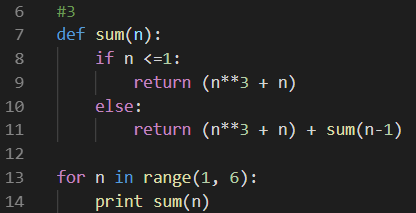
\includegraphics[scale=.8]{3a}

    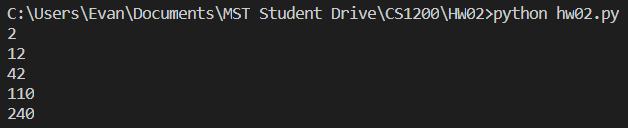
\includegraphics[scale=.8]{3b}

    %\clearpage
    \item Prove by the Principle of Recursion that
    $$\sum\limits_{i=1}^{n} i(i+1) = \frac{n(n+1)(n+2)}{3}$$
    \begin{enumerate}[1.]
        \item Define the problem.
            
            The domain for the problem is the natural numbers 1...$\infty$.
            $$f(n) = \sum\limits_{i=1}^{n} i(i+1)$$
            $$g(n) = \frac{n(n+1)(n+2)}{3}$$
            Prove $f(n) = g(n)$ for all of the domain.\\
            P(n) is true if $f(n) = g(n)$.
            
        \item 
        Check stopping values and two more.\\
        $f(1) = 1(1+1) = 2$\\
        $g(1) = \frac{1(1+1)(1+2)}{3} = 2$\\
        $f(2) = 1(1+1) + 2(2+1) = 8$\\
        $g(2) = \frac{2(2+1)(2+2)}{3} = 8$\\
        $f(3) = 1(1+1) + 2(2+1) + 3(3+1) = 20$\\
        $g(3) = \frac{3(3+1)(3+2)}{3} = 20$
        
        \item Prove recursion stays in $D$.\\
        The recursive relation is $f(n) = f(n-1) + n(n+1)$. Recursion is only 
        called if $n \geq 1$ so in all cases $n-1 \geq 0$. So, the call is 
        made with a value in $D$.

        \item Prove that recursion halts.\\
        Using the counting strategy, you can see that $n$ decreases 
        from $n$ to $n-1$, so recursion halts.
        \item Check that $P$ is inherited recursively.\\
        Assume $P(n-1)$ is true.\\
        $f(n) = f(n-1) + n(n+1)$\\
        $=g(n-1) + n(n+1)$\\
        $=\frac{(n-1)(n)(n+1)}{3} + n(n+1)$\\
        $=\frac{(n-1)(n)(n+1)}{3} + \frac{3n(n+1)}{3}$\\
        $=\frac{(n-1)(n)(n+1) + 3n(n+1)}{3}$\\
        $=\frac{(n^{3}-n)+(3n^{2}+3n)}{3}$\\
        $=\frac{n(n^{2}+3n+2)}{3}$\\
        $=\frac{n(n+1)(n+2)}{3}$\\
        $=g(n)$
        \item Conclusion\\
        After verifying steps 1-5, we can conclude that $P(n)$ is true for 
        all elements in $D$. Thus, $f(n) = g(n)$ for all real numbers.\\
        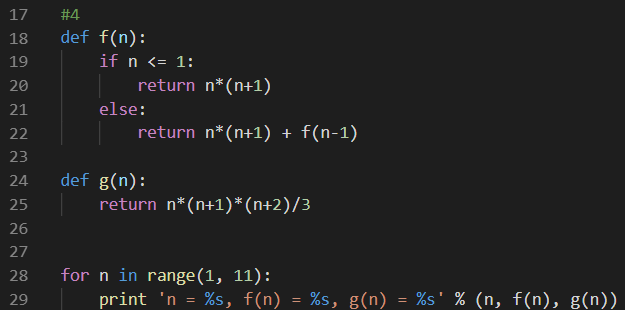
\includegraphics[scale=.8]{4a}\\
        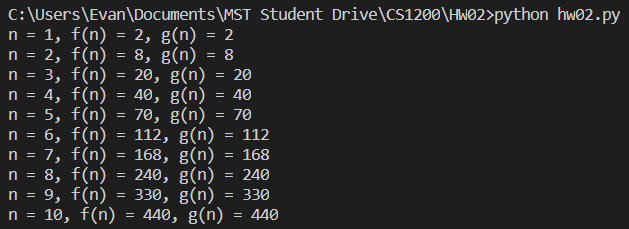
\includegraphics[scale=.8]{4b}

    \end{enumerate}
    
    \clearpage
    \item Prove by induction that for all integers $n \geq 1$
    $$1 + 6 + 11 + 16 + ... + (5n - 4) = \frac{n(5n - 3)}{2}$$
    \begin{enumerate}[1.]
        \item Define the problem.
        \begin{itemize}
            \item Domain is $1...\infty$.
            \item Prove $f(n) = g(n)$ for all of D.
            $$f(n) = 1 + 6 + 11 + 16 + ... + (5n-4)$$
            $$g(n) = \frac{n(5n - 3)}{2}$$
            \item $P(n)$ is true if $f(n) = g(n)$.
        \end{itemize}

        \item Check stopping values and two more.\\
        $f(1) = 1$\\
        $g(1) = \frac{1(1*5-3)}{2} = 1$\\
        $f(2) = 1 + 6 = 7$\\
        $g(2) = \frac{2(2*5-3)}{2} = \frac{2(7)}{2} = 7$\\
        $f(3) = 1 + 6 + 11 = 18$\\
        $g(3) = \frac{3(3*5-3)}{2} = \frac{36}{2} = 18$
        \item Inductive Case.\\
        %\begin{multicols}{2}
            $f(n) = f(n-1) + (5n-4)$\\
            $= g(n-1) + (5n-4)$\\
            $= \frac{(n-1)(5(n-1)-3)}{2} + (5n-4)$\\
            $= \frac{(n-1)(5n-5-3)}{2} + \frac{2(5n-4)}{2}$\\
            $= \frac{(n-1)(5n-8)+(10n-8)}{2}$\\
            $= \frac{5n^{2}-5n-8n+8+10n-8}{2}$\\
            $= \frac{5n^{2}-3n}{2}$\\
            $= \frac{n(5n-3)}{2}$\\
            $= g(n)$
        %\end{multicols}

        \item Conclusion.\\
        $P(n)$ is true for all of $n$ in $D$.
        Therefore $$1 + 6 + 11 + 16 + ... + (5n - 4) = \frac{n(5n - 3)}{2}$$ is true for all of $n$ in $D$.
    \end{enumerate}

    \clearpage
    \item Prove by induction that for all natural numbers $n$
    $$\sum\limits_{i=0}^{n} \frac{i^{2}}{(2i-1)(2i+1)} = \frac{n(n+1)}{2(2n+1)}$$
    \begin{enumerate}[1.]
        \item Define the problem.
            
        \begin{itemize}
            \item Domain is all natural numbers or $0...\infty$.
            $$f(n) = \sum\limits_{i=0}^{n} \frac{i^{2}}{(2i-1)(2i+1)}$$
            $$g(n) = \frac{n(n+1)}{2(2n+1)}$$
            \item Prove $f(n) = g(n)$ for all of D.
            \item $P(n)$ is true if $f(n) = g(n)$.
            
        \end{itemize}

        \item Check stopping values and two more.\\
        $f(0) = \frac{0}{(2*0-1)(2*0+1)} = 0$\\
        $g(0) = \frac{0(0+1)}{2(2*0+1)} = 0$\\
        $f(1) = \frac{1^{2}}{(2*1-1)(2*1+1)} = \frac{1}{3}$\\
        $g(1) = \frac{1(1+1)}{2(2*1+1)} = \frac{1}{3}$\\
        $f(2) = 0 + \frac{1}{3} + \frac{2^{2}}{(2*2-1)(2*2+1)} = \frac{1}{3} + \frac{4}{15} = \frac{9}{15} = \frac{3}{5}$\\
        $g(2) = \frac{2(2+1)}{2(2*2+1)} = \frac{6}{10} = \frac{3}{5}$
        \item Inductive Case.
        \begin{multicols}{2}
            $f(n)=f(n-1)+\frac{n^{2}}{(2n-1)(2n+1)}$\\
            $=g(n-1)+\frac{n^{2}}{(2n-1)(2n+1)}$\\
            $=\frac{(n-1)(n)}{2(2(n-1)+1)}+\frac{n^{2}}{(2n-1)(2n+1)}$\\
            $=\frac{n(n-1)}{2(2n-1)}+\frac{n^{2}}{(2n-1)(2n+1)}$\\
            $=\frac{n(n-1)(2n+1)}{2(2n-1)(2n+1)}+\frac{2n^{2}}{2(2n-1)(2n+1)}$\\
            $=\frac{n(n-1)(2n+1)+2n^{2}}{2(2n-1)(2n+1)}$\\
            $=\frac{2n^{3}-n^{2}-n+2n^{2}}{2(2n-1)(2n+1)}$\\
            $=\frac{2n^{3}+n^{2}-n}{2(2n-1)(2n+1)}$\\
            $=\frac{n(2n^{2}+n-1)}{2(2n-1)(2n+1)}$\\
            $=\frac{n(2n-1)(n+1)}{2(2n-1)(2n+1)}$\\
            $=\frac{n(n+1)}{2(2n+1)}$\\
            $=g(n)$
        \end{multicols}
        \item Conclusion.\\
        $P(n)$ is true for all of $n$ in $D$. Therefore 
        $$\sum\limits_{i=0}^{n} \frac{i^{2}}{(2i-1)(2i+1)} = \frac{n(n+1)}{2(2n+1)}$$ 
        is true for all of $n$ in $D$.
    \end{enumerate}
\end{enumerate}

\end{document}